\subsubsection*{Resultados obtenidos}

% \begin{figure}[H]
% 	\centering	\includegraphics[width=0.8\textwidth]{img/nombre.png}
% 	\caption{Titulo}
% 	\label{fig:etiqueta}
% \end{figure}


\begin{figure}[H]
	\centering	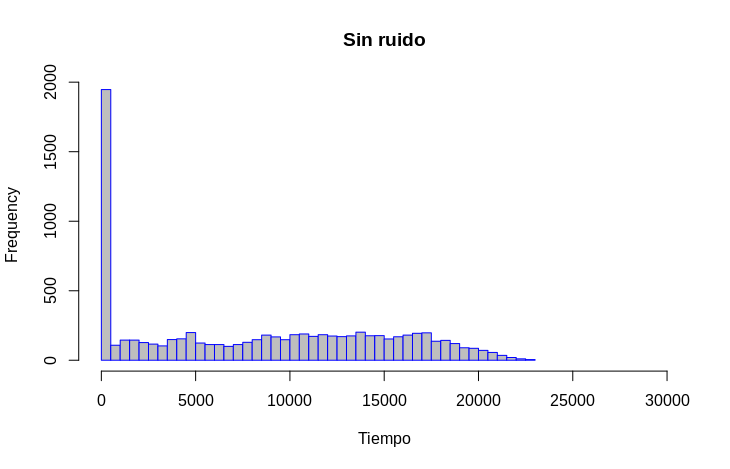
\includegraphics[width=0.8\textwidth]{img/sinRuido.png}
	\caption{Vector de tiempos de rayos sin ruido}
	\label{fig:etiqueta}
\end{figure}
\par Acá podemos observar que efectivamente, el ruido aditivo modifíca mucho más algunas partes del vector mientras que otras no se aprecian muchos cambios. En este caso el histograma de ruido aditivo sufre cambios notorios respecto del vector sin ruido, mientras que en los valores más grandes casi que no notamos se notan diferencias.

\begin{figure}[H]
	\centering	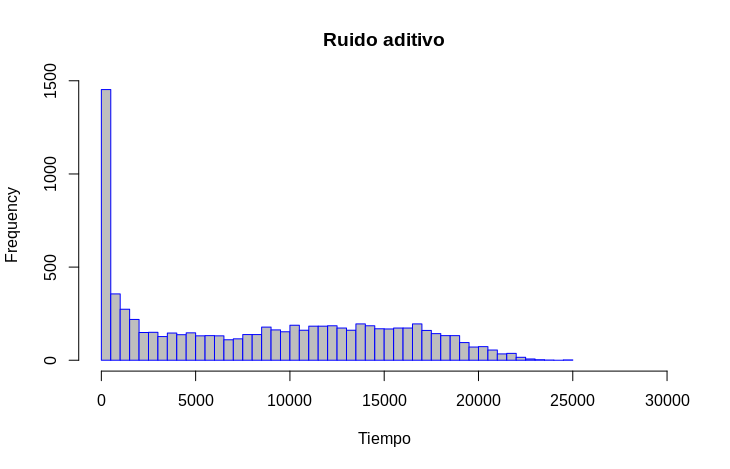
\includegraphics[width=0.8\textwidth]{img/ruidoAditivo.png}
	\caption{Vector de tiempos de rayos con ruido aditivo}
	\label{fig:etiqueta}
\end{figure}

\par En este otro caso en cambio, vemos que las diferencias entre el histograma de ruido multiplicativo y sin ruido existen pero están más uniformemente distribuídas. La única anormalidad que observamos es un incremento en los valores máximos, no obstante se trata de unos pocos casos aislados.
Esto se parece más a lo que esperabamos que hiciera nuestro ruido, por eso fue que elegimos usar este método en nuestra implementación.
\begin{figure}[H]
	\centering	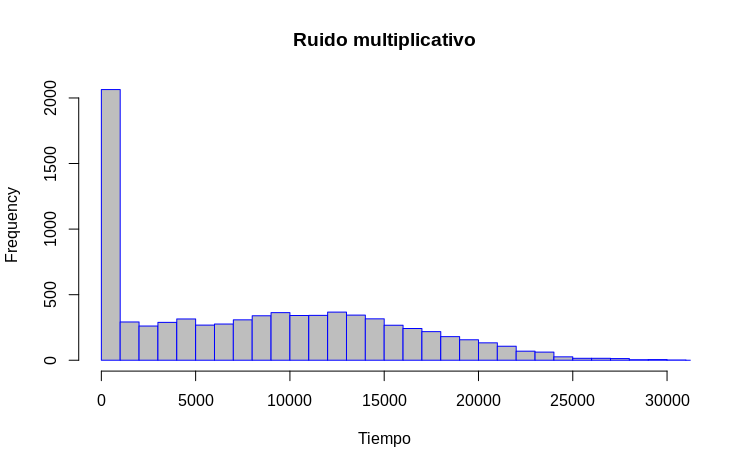
\includegraphics[width=0.8\textwidth]{img/ruidoMultiplicativo.png}
	\caption{Vector de tiempos de rayos con ruido multiplicativo}
	\label{fig:etiqueta}
\end{figure}